\section*{Appendix S4. Wannier90 bridge calculation}
\label{supp:wannier90-bridge}
\renewcommand{\theequation}{S4.\arabic{equation}}
\setcounter{equation}{0}
\renewcommand{\thetable}{S4.\arabic{table}}
\setcounter{table}{0}
\renewcommand{\thefigure}{S4.\arabic{figure}}
\setcounter{figure}{0}

\subsection*{S4.1 Role and evidence boundary}

This appendix connects the controlled gauge-locality mechanism to retained
Wannier90 executions. It does not redefine M2. The balanced calculation is the
synthetic, non-DFT record
\path{research-monograph.periodic-2d.wannier90-balanced.v1} under
\path{calculations/research-monograph/periodic-2d/}. The parent is a finite
plane-wave representation of
\begin{equation}
 H=-\nabla^2+0.5\cos x+0.5\cos y+0.15\cos x\cos y
 \label{eq:supp-s4-parent}
\end{equation}
with a $15\times15\times1$ reciprocal mesh and a retained lowest-three-band
subspace. Wannier90 3.1.0 used centered $s$, $p_x$, and $p_y$ trial
projections; no disentanglement was used.

The external execution was historically authorized and retained. It is not
rerun by this manuscript. Repository-only verification consumes the compact
portable fixture and reconstructs the comparison independently of the
extractor. Passing establishes bounded consistency for this synthetic finite
interface, not first-principles, material, or general Wannier90 validation.

\subsection*{S4.2 Converged finite case and common-space alignment}

After a retained failed preprocessing attempt, the balanced auxiliary embedding
completed preprocessing and localization. Localization satisfied the frozen
$10^{-12}$ spread criterion at iteration 94. The direct projected frame and the
Wannier90 frame span the same retained subspace within a maximum projector
Frobenius defect of $2.65\times10^{-10}$.

Their raw represented Hamiltonians differ by $1.137E_G$ in maximum Frobenius
norm. Let $U_{\mathrm d}(\bm k)$ and $U_{\mathrm W}(\bm k)$ denote the direct
and Wannier90 frames. The pointwise unitary identification derived from those
frames reduces the represented-operator defect to
$3.57\times10^{-10}E_G$. By contrast, the frozen bounded family consisting of
independent integer orbital translations in $[-1,1]^2$ followed by one constant
orbital unitary leaves a per-orbital frame RMS defect of $1.188$ and an operator
defect of $1.490E_G$. Thus the observed relation is genuinely
$\bm k$-dependent within this comparison contract; it is not explained by a
single orbital rotation and bounded relabeling of orbital cells.

\subsection*{S4.3 Localization and hopping locality}

Native Wannier90 Berry-link spreads and common finite-supercell spreads use
different estimators and are not substituted for one another. The native total
active-plane spread is $0.7094a^2$. Under the common finite-supercell estimator,
the Wannier90 total is $6.1359a^2$ and the direct projected total is
$24.5163a^2$, giving a ratio of $0.2503$ for this finite case.

The same frame change also affects matrix-hopping tails. At squared-radius
shell 18, the omitted Frobenius $\ell^2$ norm is
$9.92\times10^{-3}E_G$ for the Wannier90 frame and
$1.38\times10^{-2}E_G$ for the direct projected frame. At shell 50 the values
are $2.72\times10^{-4}E_G$ and $5.90\times10^{-3}E_G$, respectively. These
commensurate diagnostics support the expected connection between localized
frames and shorter represented hopping tails for the frozen case. They do not
establish an optimality theorem.

The native \path{_hr.dat} blocks reconstruct the external mesh within
$3.06\times10^{-5}E_G$ in maximum Frobenius norm and
$2.23\times10^{-5}E_G$ spectrally. Those defects are retained as finite decimal
serialization effects, not relabeled as hopping truncation.

\begin{figure}[t]
 \centering
 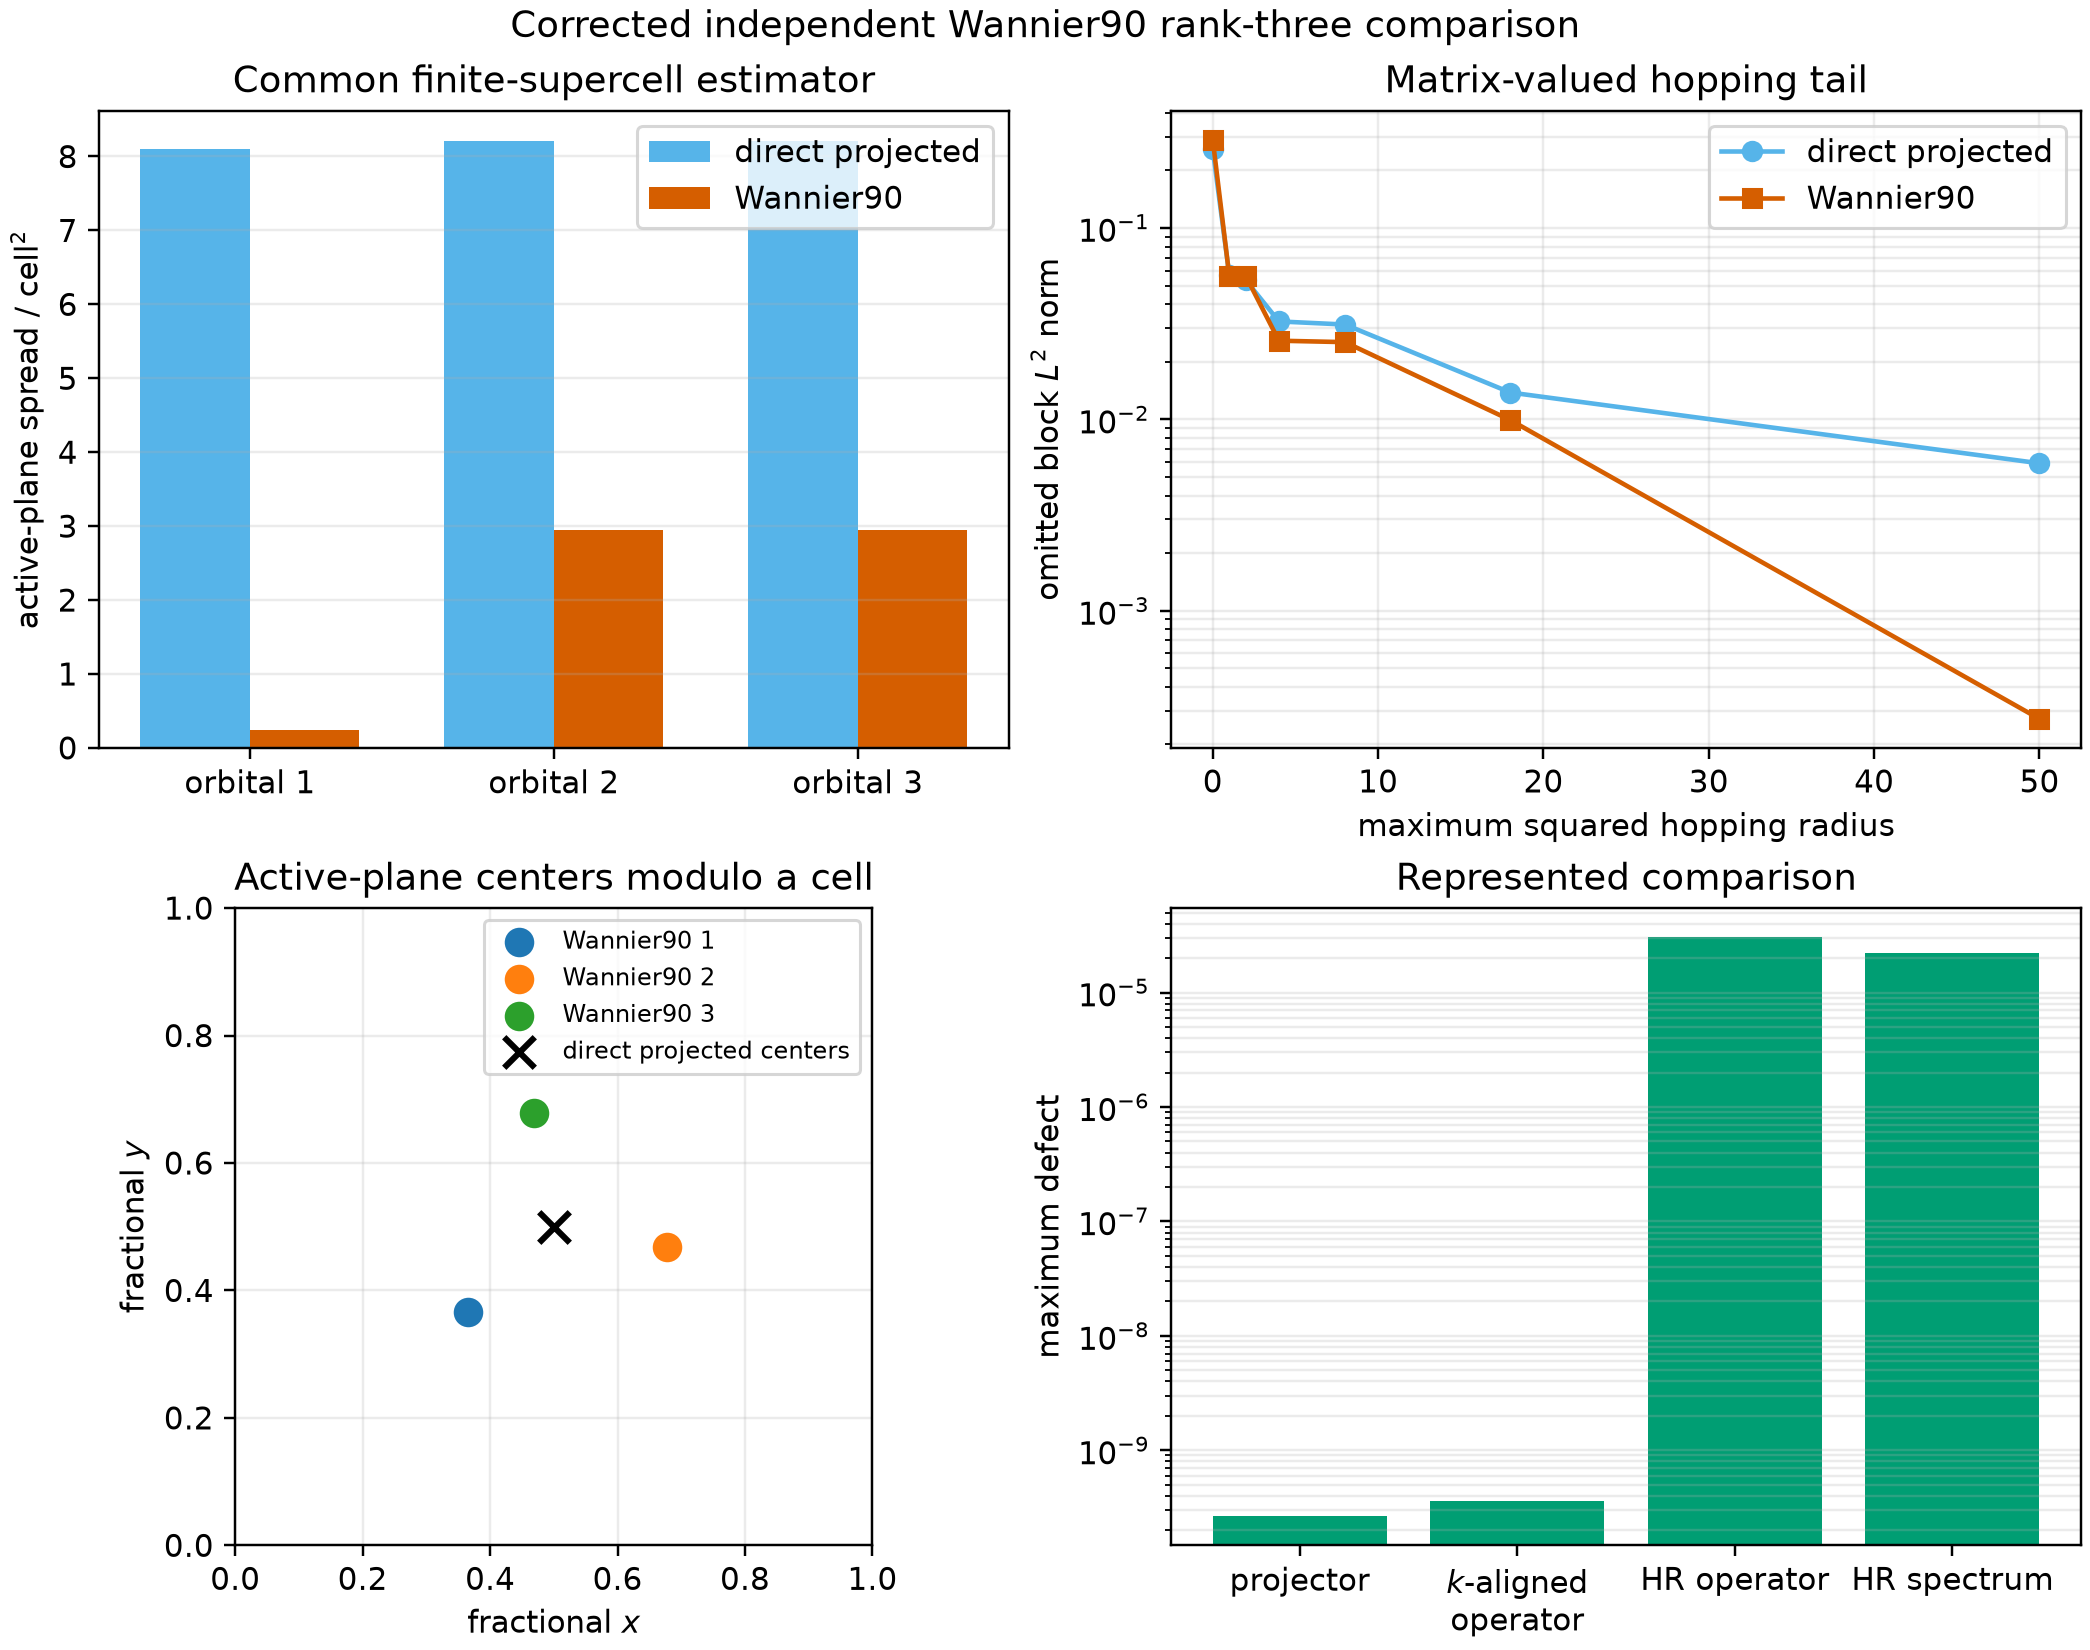
\includegraphics[width=0.97\linewidth]{../../../../../calculations/research-monograph/periodic-2d/wannier90-balanced-summary.png}
 \caption{Retained balanced Wannier90 comparison. Native and common-estimator
 spreads remain separate; aligned operator and shell-tail channels are evaluated
 on declared common representations.}
 \label{fig:supp-s4-wannier90-balanced}
\end{figure}

\subsection*{S4.4 Sensitivity study and interpretation limit}

A separately retained six-case study varies one of reciprocal mesh, plane-wave
cutoff, or inactive embedding length at a time. All finite cases converged, but
the outcomes are nonmonotone. Table~\ref{tab:supp-s4-sensitivity} records the
native spread and radius-50 tail needed for the interpretation boundary.

\begin{table}[t]
\centering
\small
\caption{Selected retained Wannier90 sensitivity observations.}
\label{tab:supp-s4-sensitivity}
\begin{tabular}{@{}lrr@{}}
\toprule
Case & Native spread ($a^2$) & Radius-50 tail ($E_G$)\\
\midrule
Reference $P3,N15,c15$ & $0.7094$ & $2.72\times10^{-4}$\\
Mesh $N=19$ & $1.7901$ & $4.52\times10^{-2}$\\
Cutoff $P=2$ & $1.7072$ & $3.30\times10^{-2}$\\
Cutoff $P=4$ & $1.7024$ & $3.38\times10^{-2}$\\
Embedding $c=12$ & $0.7093$ & $2.72\times10^{-4}$\\
Embedding $c=18$ & $1.7024$ & $3.38\times10^{-2}$\\
\bottomrule
\end{tabular}
\end{table}

The $c=12$ case returns close to the reference, whereas $c=18$ reaches a
different localization basin. The cutoff and mesh observations likewise do not
form a convergence sequence. Accordingly, the balanced calculation is a
positive finite-case bridge between M2's gauge mechanism and an actual
Wannier90-selected frame, while the sensitivity study blocks any claim of
mesh-, cutoff-, embedding-, or basin-independent localization. Neither record
supports a Si:P, Si:B, bulk-silicon, or other material-specific locality bound.

\subsection*{S4.5 Verification and provenance}

The portable balanced verifier independently reconstructs the finite parent,
direct polar frame, subspace and represented-operator defects, bounded
translation-plus-constant alignment search, native hopping reconstruction,
shell tails, convergence record, and common-grid densities and spreads. The
portable sensitivity verifier checks all six retained cases. Both pass against
the retained records. The directory-level \path{SHA256SUMS} manifest verifies
the reports, results, portable evidence, scripts, and figures. As in Appendix
S2, the digests establish byte consistency relative to the retained manifest;
they are not by themselves an external timestamp or a material-validation
argument.
